\documentclass{beamer}
\usepackage{hyperref}
\usepackage{subfig}  %% Para incluir subgraficos
\usepackage{graphicx}
\usepackage{media9} % 
\usepackage{url}
\usepackage{ragged2e}  % Allow justification
\usepackage[margin=20pt,font=small,labelfont=bf,labelsep=period]{caption}

\usepackage[spanish, activeacute]{babel}
\usepackage[utf8]{inputenc}
\decimalpoint
%\usepackage{natbib}

%
\hypersetup{pdfstartview={Fit}, bookmarks=True, pdftitle={SCEC Presentation}, pdfauthor={Juan Carlos Vergara-Gallego}, pdfsubject={Presentation}, pdfkeywords={Waves, Elasticity, Numerical Methods, High Performance Computing, BEM}, pdfpagemode=UseOutlines, bookmarks, bookmarksopen, pdfstartview=FitH, colorlinks,linkcolor=blue, urlcolor=black, citecolor=blue}  % Configure hyperref

%--- New commands ----%
\newcommand{\footref}[1]{\textsuperscript{\ref{#1}}}
\newcommand{\pardiff}[2]{\frac{\partial #1}{\partial #2}}
\newcommand{\pardiffd}[2]{\frac{\partial^2 #1}{\partial #2^2}}
%
%---------------------%
%\usefonttheme[onlymath]{serif}  % Make equations to be in serif fonts
\usefonttheme{serif}  % Make equations to be in serif fonts

\begin{document}


%title
\title[CyberShake] % (optional, only for long titles)
{A Physics-Based Seismic Hazard Model for Southern California}
\subtitle{CyberShake, Southern California Earthquake Center}
\author[Vergara Gallego, Juan Carlos] % (optional, for multiple authors)
{Juan Carlos Vergara Gallego\\ \texttt{\small jvergar2@eafit.edu.co}\\
{\tiny Presentación disponible en: \url{https://github.com/jvergar2/03_SCEC}}}
\institute{Departamento de Ingeniería Civil\\
  Universidad EAFIT}
\date{\today}
\subject{Ingeniería Sísmica}

% Title page
\frame{\titlepage}

% Outline
\begin{frame}
	\frametitle{Outline}
	\tableofcontents
\end{frame}
%
%
\section{Introduction}
\begin{frame}
\frametitle{Introducción}
%
\justifying
Se presenta un resumen del proyecto {C}yber{S}hake, de sus objetivos y la foma como están abordando el problema de construir el modelo de Amenaza en el Sur de California.

\url{http://scec.usc.edu/scecpedia/CyberShake}
%
\end{frame}
%
%
\begin{frame}[allowframebreaks]
\frametitle{¿Qué es el CyberShake?}
%
\justifying
{C}yber{S}hake, es un proyecto de investigación del ``Southern California Earthquake Center's" (SCEC), dentro del cual se encuentran desarrollando un modelo computacional a gran escala para incluir determinísticamente el efecto de la fuente y la ruta de propagación de las ondas sísmicas en la amenaza sísmica del Sur de California.
%
\end{frame}
%\transwipe
%
\begin{frame}
\frametitle{¿Qué es el CyberShake?}
\begin{figure}[h]
	\centering
	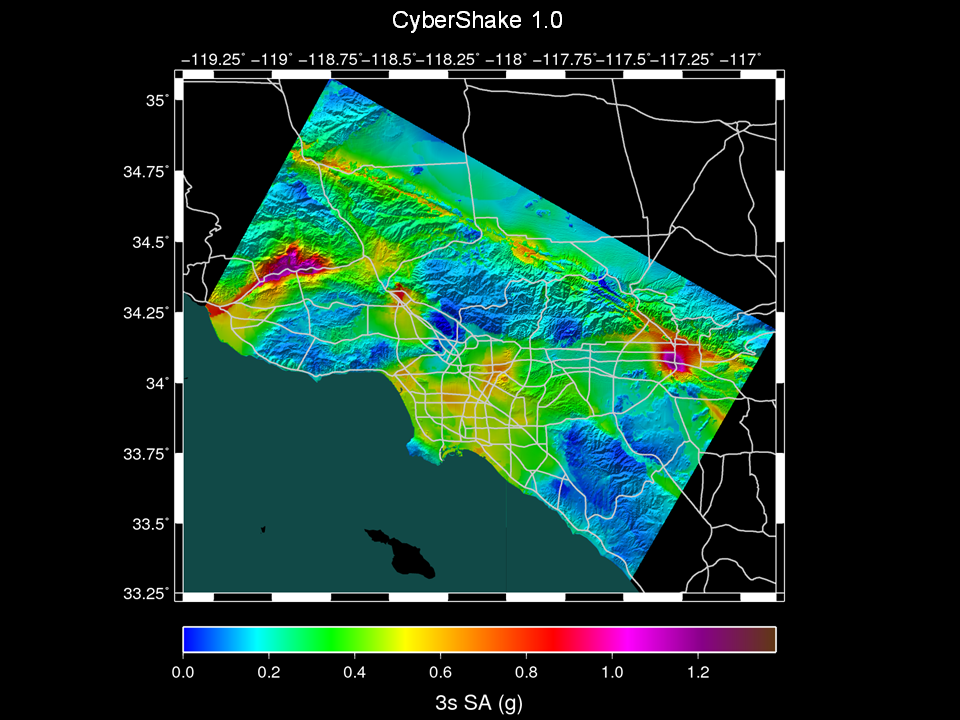
\includegraphics[height=6cm]{img/CyberShake_2009.PNG}
	\caption{Mapa de amenaza sísmica del Sur de California calculado con CyberShake. \footnote{\url{http://scec.usc.edu/scecwiki/images/6/61/CandB_2008.PNG}\\}}
\end{figure} 
%
\end{frame}
%
%
\begin{frame}
\frametitle{¿Qué es el CyberShake?}
%
\begin{figure}[h]
	\centering
	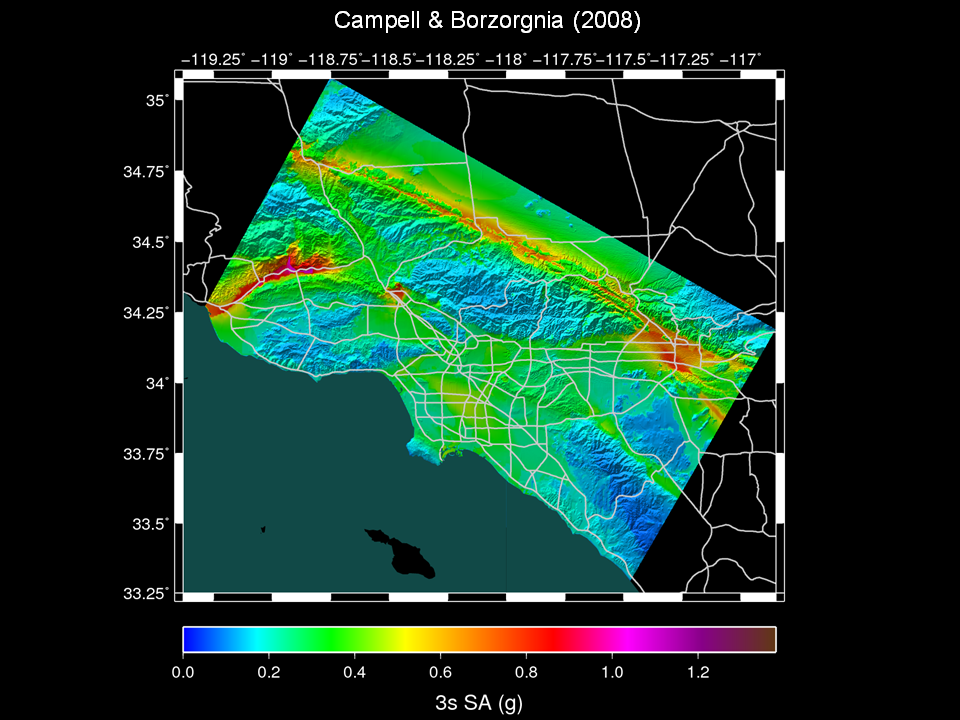
\includegraphics[height=6cm]{img/CandB_2008.PNG}
	\caption{Mapa de amenaza sísmica del Sur de California calculado con las ecuaciones de predición del movimiento del suelo (GMPE). \footnote{\url{http://scec.usc.edu/scecwiki/images/6/61/CandB_2008.PNG}\\}}
\end{figure}
%
%
%\begin{figure}[h]
%\centering
%%
%	\subfloat[Ricker pulse.]{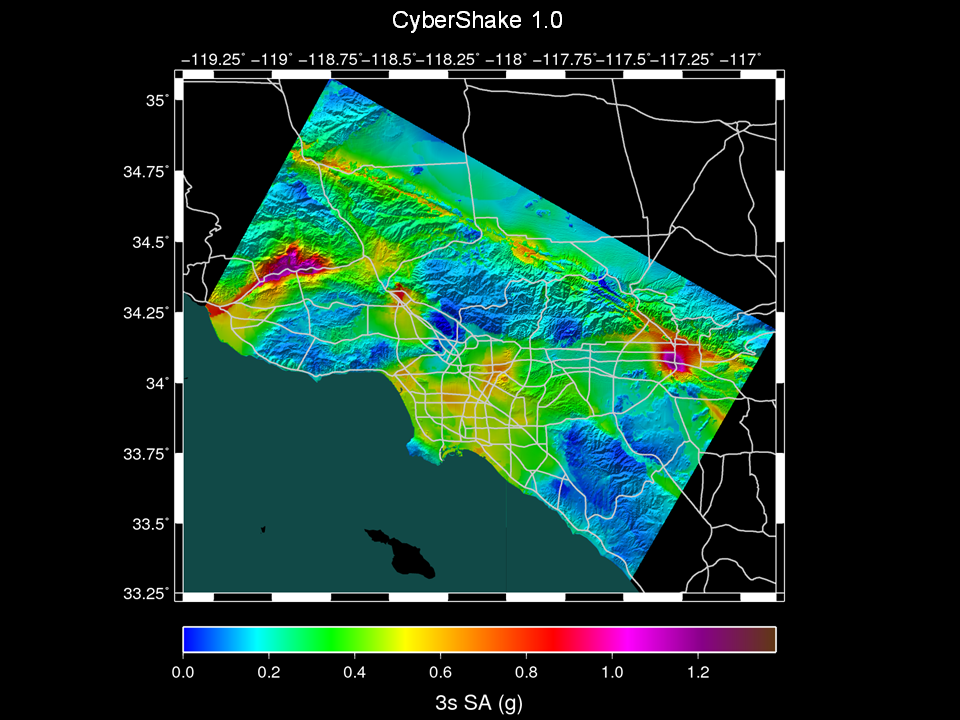
\includegraphics[width=0.4\textwidth]{img/CyberShake_2009.PNG}}\qquad
%	%
%	\subfloat[Ricker pulse spectrum.]{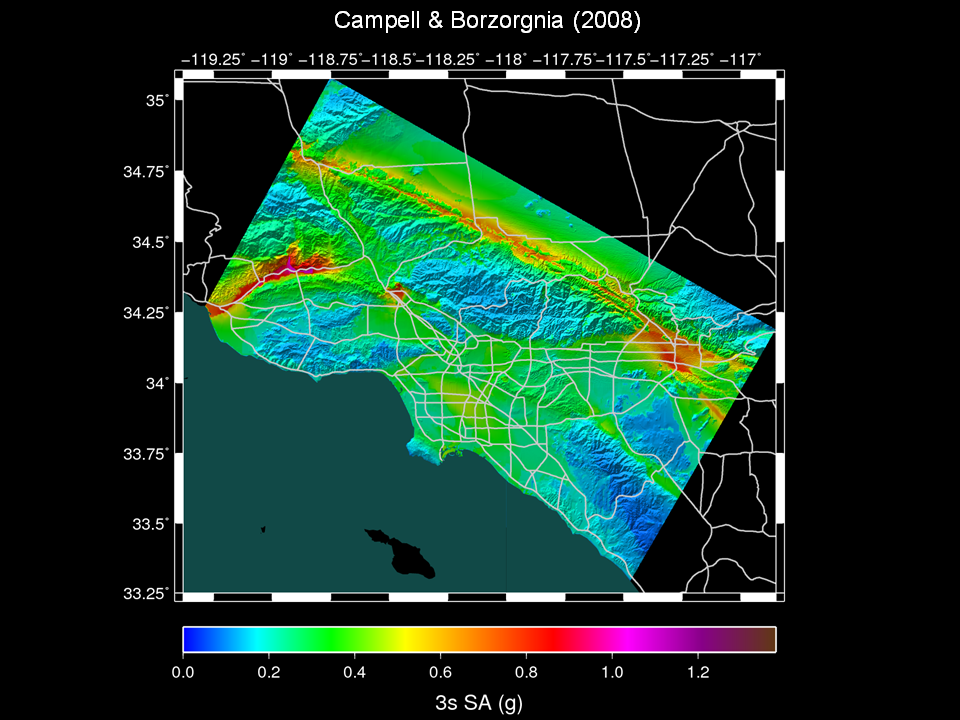
\includegraphics[width=0.4\textwidth]{img/CandB_2008.PNG}}
%	%
%\caption{Ricker pulse and its spectrum.}
%
%\end{figure}
\end{frame}
%
%
\section{¿Qué se hace actualmente?}
\begin{frame}[allowframebreaks]\frametitle{Ground Motion Prediction Equations}
%
Acá voy a meter un texto que me va a pasar La Morsa.
%
%
\begin{figure}[h]
	\centering
	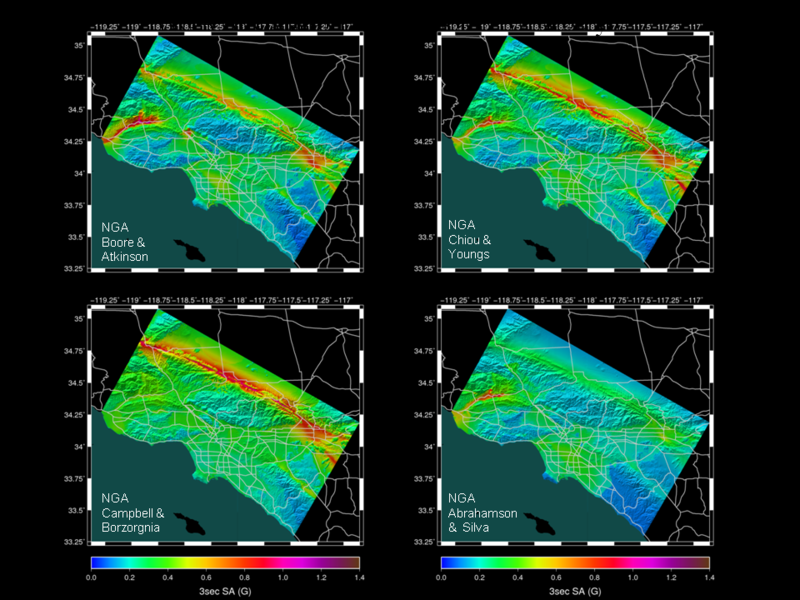
\includegraphics[height=3cm]{img/UCERF2_GMPE_2007.PNG}
	\caption{Mapa de amenaza sísmica del Sur de California calculado con cautro ecuaciones de predición del movimiento del suelo (GMPE) diferentes. \footnote{\url{http://scec.usc.edu/scecwiki/images/b/bd/UCERF2_GMPE_2007.PNG}\\}}
\end{figure}
%
A pesar de que las cuatro leyes de atenuación son aceptadas en la comunidad científica, es evidente las grandes diferencias entre ellas.
%
\end{frame}
%
%
\section{¿Con que información cuentan?}
\subsection{UCERF $2.0$ y $3.0$}
\begin{frame}[allowframebreaks]
\frametitle{Uniform California Earthquake Rupture Forecast, Version $2.0$ y $3.0$ (UCERF $2.0$ y $3.0$)}
%
\justifying
%
El $UCERF3.0$ estima la probabilidad de ocurrencia de sismos, para una magnitud específica y localización, que pueden ocurrir dentro de una ventana de tiempo en California EE.UU. La versión $3.0$ es una mejora de la versión $2.0$, dando la posibilidad de la ruptura simultanea de varias fallas y mejorando la sobre-estimación que daba $UCERF2.0$ para magnitudes entre $6.5$ y $7.0$.\\
%
Cuantro componentes básicos de $UCERF3.0$:
%
	\begin{itemize}
	\justifying
	%
		\item Modelo de Falla: Geometría física de las fallas conocidas.
		%
		\item Modelo de Deformación: ``Taza de deslizamiento" de cada sección de la falla. Con esto se calcula el momento sísmico.
		%
		\item ``Earthquake Rate Model": Taza de todos los sismos dentro de una región sobre una magnitud mínima especificada.
		%
		\item Modelos de Probabilidad: Determina la probabilidad de ocurrencia de cada evento dentro de una ventana de tiempo.
	%
	\end{itemize}
%
\begin{figure}[h]
	\centering
	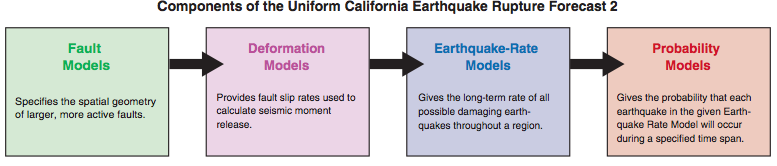
\includegraphics[height=1.75cm]{img/Components_UCERF.png}
	\caption{Componentes básicos del modelo UCERF3.0. \cite[figura 2, página 7]{ucerf3}}
\end{figure}
%
%
Con la información suministrada por $UCERF2.0$ se identifican todas las posibles fallas sísmicas $200$ $km$ dentro de la región de estudio. Todas las fallas se usan para generar diferentes escenarios, dentro de los cuales se varía la ubicación del hypocentro y la forma de la ruptura.\\
%
En total se generan al rededor de $415.000$ escenarios de ruptura para cada sitio. 
%
%
%\end{frame}
%%
%%
%\begin{frame}[allowframebreaks]
%\frametitle{Uniform California Earthquake Rupture Forecast, Version $2.0$ y $3.0$ (UCERF $2.0$ y $3.0$)}
%
\begin{figure}[h]
	\centering
	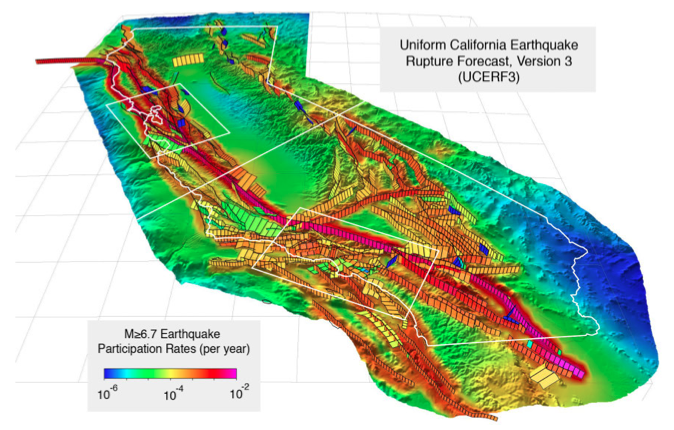
\includegraphics[height=6cm]{img/UCERF3_Map.png}
	\caption{Mapa $3D$ de California, mostrando las $2606$ fallas mapeadas en $UCERF3.0$ \cite[figura 1, página 5]{ucerf3}}
\end{figure}
%
\end{frame}
%
%
\subsection{Modelos de Velocidad}
\begin{frame}[allowframebreaks]
\frametitle{SCEC Community Velocity Model: CVM-S.}
%
\justifying
%
El modelo de velocidad comunitario de California (CVM-S \footnote{Actualmente se encuentra disponible en linea la versión $4.0$ de dicho modelo. \url{http://www.data.scec.org/research-tools/3d-velocity.html}, \url{http://scec.usc.edu/scecpedia/CVM-S}, último acceso $03$ de Octubre de $2014$.}, por sus siglas en ingles), tiene como propósito servir como modelo de referencia en varias áreas de investigación que dependen de las estrucutras, propiedades de los materiales tales como la velocidad de propagación de las ondas sísmicas, en profundidad para llevar acabo diferentes análisis. Las velocidades de mayor profundidad se construye con base reglas que relacionan la profundidad y la edad de los depósitos sedimentarios con las velocidades de las ondas sísmicas. Las velocidades de propagación en los depósitos menos profundos son tomadas de las medidas de los estudios geotécnicos. Las velocidades de propagación en roca son tomados de estudios tomográficos.\\
%
El modelo de velocidad CVM-S es de libre acceso, un usuario puede obtener los códigos escritos en Fortran, compilarlos y ejecutarlos en una máquina personal. El código se alimenta con un archivo de texto que contiene la latitud, longitud y profundidad de puntos donde se quiere conocer $V_p$, $V_s$ y la densidad.
%
%
\begin{figure}[h]
	\centering
	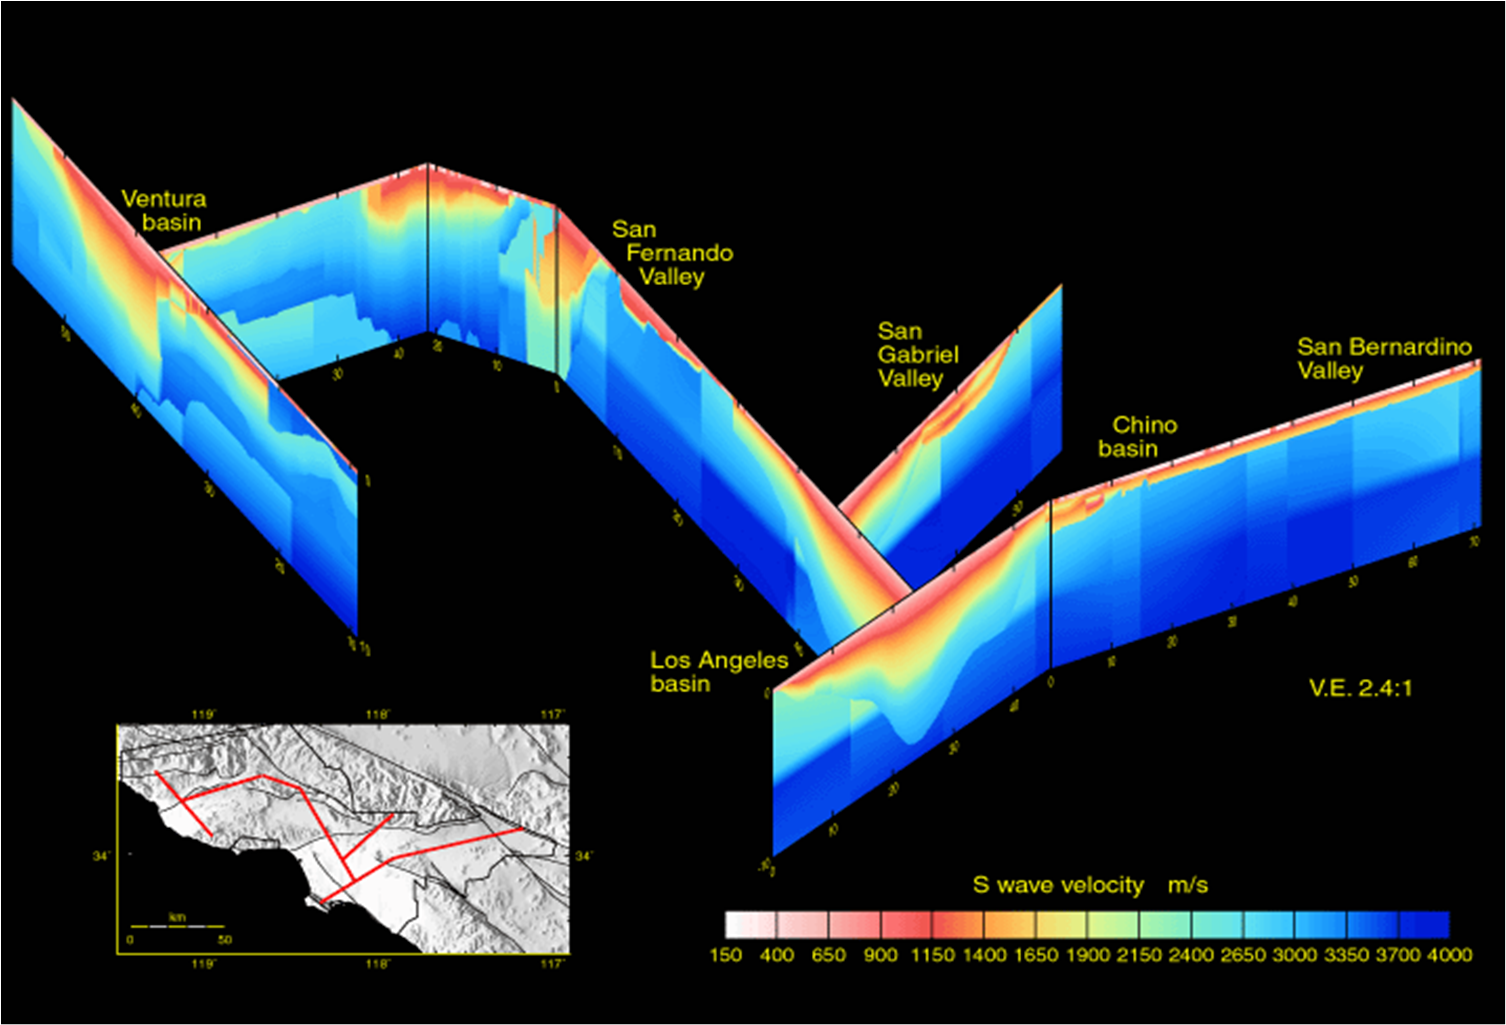
\includegraphics[height=6cm]{img/CVM-S4.png}
	\caption{Secciones transversales de California mostrando la variación en profundidad de la velocidad. \footnote{\url{http://scec.usc.edu/scecwiki/images/a/a7/CVM-S4.png}}}
\end{figure}
%
\end{frame}
%
%
\begin{frame}[allowframebreaks]{References}
\def\newblock{}
%\bibliographystyle{gji}
%\bibliography{refSCEC}
\bibliographystyle{plain}
\begin{thebibliography}{1}

\bibitem{book:aki} Keiiti Aki \& Paul G. Richards. {Q}uantitative {S}eismology. University Sciencie Books, 2nd Edition, Mill Valley, San Diego, 2002.

\bibitem{gravesetal} Graves, R.; Jordan, T. H.; Callaghan, S.; Deelman, E.; Field, E.; Juve, G.; ... \& Vahi, K. (2011). CyberShake: A physics-based seismic hazard model for southern California. Pure and Applied Geophysics, 168(3-4), 367-381.

\bibitem{ucerf2} Field, E. H., Dawson, T. E., Felzer, K. R., Frankel, A. D., Gupta, V., Jordan, T. H., ... \& Wills, C. J. (2009). Uniform California earthquake rupture forecast, version 2 (UCERF 2). Bulletin of the Seismological Society of America, 99(4), 2053-2107.

\bibitem{ucerf3} Field, E.H., Biasi, G.P., Bird, P., Dawson, T.E., Felzer, K.R., Jackson, D.D., Johnson, K.M., Jordan, T.H., Madden, C., Michael, A.J., Milner, K.R., Page, M.T., Parsons, T., Powers, P.M., Shaw, B.E., Thatcher, W.R., Weldon, R.J., II, and Zeng, Y., 2013, Uniform California earthquake rupture forecast, version 3 (UCERF3)—The time-independent model: U.S. Geological Survey Open-File Report 2013–1165, 97 p., California Geological Survey Special Report 228, and Southern California Earthquake Center Publication 1792, \url{http://pubs.usgs.gov/of/2013/1165/}.

\bibitem{wiki:FVM} Finite volume method. (2014, April 22). In Wikipedia, The Free Encyclopedia. Retrieved 00:44, September 25, 2014, from \url{http://en.wikipedia.org/w/index.php?title=Finite_volume_method&oldid=605282055}

\end{thebibliography}

\end{frame}


\end{document}

